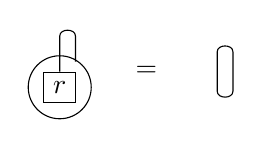
\begin{tikzpicture}
    \coordinate(origin1)at(0,0);
    \node at(1.1,0)[anchor=center]{$=$};
    \coordinate(origin2)at(2,-.25);
    \draw
    (origin1)node[anchor=north,draw,rectangle](r2){$\bm{r}$}
    (r2.center)circle[radius=.4]
    (r2.north)--++(0,.45)
    .. controls ++(0,.1) and ++(0,.1) .. ++(.2,0)
    --++(0,-.325)
    ;
    \draw
    (origin2)--++(0,.5)
    .. controls ++(0,.1) and ++(0,.1) ..++(.2,0)
    --++(0,-.5)
    .. controls ++(0,-.1) and ++(0,-.1) .. ++(-.2,0)
    ;
\end{tikzpicture}
